% =====================================
% 01 - PREAMBULE / PENGATURAN AWAL
% =====================================
\documentclass[aspectratio=179]{beamer}
\usetheme[progressbar=frametitle,block=fill]{metropolis} 
\setbeamertemplate{footline}{}  % Code uhtuk menghilngkan nomor pada halaman 

\usepackage[utf8]{inputenc}
\usepackage{graphicx}    % untuk gambar
\usepackage{tikz}        % untuk elemen visual
\usepackage{fontawesome5} % ikon FontAwesome
% \usepackage{quote}       % untuk gaya kutipan

% =====================================
% 02 - INFORMASI JUDUL
% =====================================
\title {Pengenalan ITIL Foundation}
\subtitle{Key Concepts of Service Management}

\author{
  \faUsers\ \textbf{Kelompok 1} 
  \begin{columns}
    \column{0.6\textwidth}
      \begin{tabular}{ll}
        Rohmat Cahyo Susilo     & (225510019) \\ 
        Muhammad Rifki Nuryasin   & (225510018) \\
        Asyrof Hafizh Maulana    & (225510003) \\
        Johan Maulana   & (225510014) \\
        Ludang Prasetyo Nugroho  & (225510017) \\
      \end{tabular}
    \column{0.3\textwidth}
      
\includegraphics[width=0.9\linewidth]{UTDI.png} % Ukuran gambar diperkecil
  \end{columns}
    }

\institute{\faUniversity\ Universitas Teknologi Digital Indonesia (UTDI)}
\date{\faCalendar\ \today}

% =====================================
% 03 - MULAI DOKUMEN
% =====================================
\begin{document}
\maketitle

% =====================================
% 04 - DAFTAR ISI
% =====================================
\begin{frame}{\faList\ Daftar Isi}
  \begin{itemize}
    \item  \textbf{Pendahuluan}
    \item  \textbf{Nilai dan Penciptaan Nilai Bersama}
    \item  \textbf{Organisasi, Penyedia Layanan, Konsumen Layanan, dan Pemangku Kepentingan Lainnya}
    \item  \textbf{Produk dan Layanan}
    \item  \textbf{Komponen Sistem Nilai Layanan ITIL}
    \item  \textbf{Nilai: Hasil, Biaya, dan Risiko}
    \item  \textbf{Penutup}
  \end{itemize}
\end{frame}

% =====================================
% 05 - SECTION 1: Pendahuluan
% =====================================
\section{Pendahuluan}
\begin{frame}{\faInfoCircle\ Pendahuluan}
   \begin{block}{Mengapa ITIL Penting?}
     \textbf{Pemahaman konsep ITIL sangat penting untuk mengatasi tantangan dalam manajemen layanan.}
     Konsep utamanya meliputi nilai, pemangku kepentingan, layanan, hubungan layanan, serta hasil, biaya, dan risiko. 
     Semua ini membantu organisasi menciptakan nilai melalui layanan.
   \end{block}
\end{frame}

\begin{frame}{\faInfoCircle\ \textbf{Pendahuluan}}
  \begin{block}{Manfaat ITIL}
    \begin{itemize}
      \item \faCheckCircle\ \textbf{Menyelaraskan layanan TI} dengan kebutuhan bisnis agar lebih efektif dan efisien.
      \vspace{0.3em}
      \item \faRocket\ \textbf{Mendukung inovasi dan kecepatan} dalam pengembangan serta penerapan layanan baru.
      \vspace{0.3em}
      \item \faSync\ \textbf{Mempercepat transformasi digital} melalui pendekatan layanan yang terstruktur dan adaptif.
    \end{itemize}
  \end{block}

  \vfill
  \centering
  \textit{\small Dengan ITIL, organisasi lebih siap menghadapi perubahan teknologi dan kebutuhan pelanggan.}
\end{frame}

% =====================================
% 06 - SECTION 2: Nilai dan Penciptaan Nilai Bersama
% =====================================
\section{Nilai dan Penciptaan Nilai Bersama}
\begin{frame}{Nilai dan Penciptaan Nilai Bersama}

    \begin{block}{Tujuan Utama Organisasi}
    {Tujuan utama dari sebuah organisasi adalah menciptakan nilai bagi para pemangku kepentingan. Nilai dalam konteks ini didefinisikan sebagai manfaat, kegunaan, dan pentingnya suatu hal yang dirasakan oleh pengguna layanan.}
    \end{block}
  
\end{frame}

\begin{frame}{Nilai dan Penciptaan Nilai Bersama}
   \begin{block}{Konsep Penciptaan Nilai Bersama}
      {Dulu, penyedia layanan dianggap sebagai pihak yang “mengirimkan” nilai ke konsumen secara sepihak. Namun, pendekatan ini sudah ketinggalan zaman. Kini, nilai dianggap diciptakan secara bersama-sama (co-created) melalui kolaborasi aktif antara penyedia dan konsumen layanan.\\Contohnya:}

  \begin{itemize}
      \item Konsumen tidak lagi hanya menerima layanan, tapi juga terlibat dalam proses penyediaan nilai.
      \item Interaksi antara penyedia dan pengguna sangat penting untuk memahami kebutuhan dan harapan.
  \end{itemize}
  \end{block}
\end{frame}

\begin{frame}{Nilai dan Penciptaan Nilai Bersama}
  \begin{block}{Untuk menjadi kolaborator yang kreatif dalam rantai nilai layanan, para pemangku kepentingan di seluruh rantai nilai layanan berkontribusi dalam mendefinisikan kebutuhan, merancang solusi layanan, bahkan hingga pada proses penciptaan dan/atau penyediaan layanan itu sendiri.}
  {Nilai akan dibahas lebih mendalam di bagian selanjutnya dalam bab ini. Namun, sebelum itu penting untuk menjelaskan siapa saja para pemangku kepentingan yang terlibat dalam penciptaan nilai bersama serta istilah-istilah yang digunakan dalam ITIL untuk menggambarkan mereka.}
  \end{block}
\end{frame}

% =====================================
% 07 - SECTION 3: Organisasi, Penyedia Layanan, Konsumen Layanan, dan Pemangku Kepentingan Lainnya
% =====================================
\section{Organisasi, Penyedia Layanan, Konsumen Layanan, dan Pemangku Kepentingan Lainnya}
\begin{frame}{Organisasi, Penyedia Layanan, Konsumen Layanan, dan Pemangku Kepentingan Lainnya}

    \begin{block}{Pengertian Organisasi}
    \begin{itemize}
        \item Organisasi adalah individu atau kelompok yang memiliki fungsi, tanggung jawab, kewenangan, dan hubungan untuk mencapai tujuan tertentu.
        \item Organisasi bisa berupa satu orang, tim, atau jaringan kompleks dari entitas hukum.
        \item Peran organisasi bisa berbeda tergantung konteks; bisa jadi penyedia layanan atau konsumen layanan.
    \end{itemize}
    \end{block}
  
\end{frame}

\begin{frame}{Organisasi, Penyedia Layanan, Konsumen Layanan, dan Pemangku Kepentingan Lainnya}
\begin{block}{Penyedia Layanan (Service Provider)}
    {Dalam pandangan tradisional ITSM, organisasi penyedia biasanya adalah departemen IT dalam perusahaan, sedangkan departemen lainnya dianggap sebagai konsumen. Namun, ini hanyalah model sederhana. Penyedia juga bisa menjual layanan di pasar terbuka, kepada bisnis lain, konsumen individual, atau menjadi bagian dari aliansi layanan yang bekerja sama dalam menyediakan layanan kepada organisasi konsumen. Yang terpenting adalah organisasi dalam peran penyedia harus memahami siapa konsumennya dan siapa pemangku kepentingan lainnya dalam hubungan layanan tersebut.}
\end{block}
\end{frame}

\begin{frame}{Organisasi, Penyedia Layanan, Konsumen Layanan, dan Pemangku Kepentingan Lainnya}
  \begin{block}{Konsumen Layanan (Service Consumer)}
    \textbf{Jenis-jenis Peran Konsumen:}
    \begin{itemize}
        \item Customer: Menentukan kebutuhan layanan dan bertanggung jawab atas hasil penggunaannya.
        \item User: Pengguna langsung layanan.
        \item Sponsor: Pihak yang menyetujui dan membiayai layanan.
    \end{itemize}
    \textbf{Contoh Kasus: Layanan Telepon Seluler}
    \begin{itemize}
        \item CIO → Customer: Menentukan kebutuhan dan mengawasi layanan.
        \item CFO → Sponsor: Menyetujui anggaran layanan.
        \item Pegawai → User: Menggunakan layanan.
    \end{itemize}
  \end{block}
\end{frame}

\begin{frame}{Organisasi, Penyedia Layanan, Konsumen Layanan, dan Pemangku Kepentingan Lainnya}
 \begin{block}{Pemangku Kepentingan Lainnya}
     {Layanan tidak hanya diciptakan oleh penyedia dan konsumen, tapi juga oleh stakeholder lainnya.\\
     Contoh stakeholder: 
     \begin{itemize}
         \item pegawai internal
         \item mitra
         \item pemasok
         \item investor
         \item pemerintah dan masyarakat.
     \end{itemize}
}
 \end{block}
    
\end{frame}

\begin{frame}{Organisasi, Penyedia Layanan, Konsumen Layanan, dan Pemangku Kepentingan Lainnya}
    \begin{block}{Pentingnya Stakeholder:}
        {Hubungan yang baik dengan stakeholder penting untuk keberhasilan dan kelangsungan organisasi.\\
        Contoh Nilai bagi Stakeholder (Tabel Ringkasan):\\
        }
        \begin{tabular}{|c|c|}
        \hline 
        \textbf{Stakeholder} & \textbf{Contoh Nilai} \\ \hline
        Konsumen Layanan & Manfaat, biaya dan risiko yang optimal  \\ \hline
        Penyedia Layanan & Dana dari konsumen, pengembangan bisnis, peningkatan citra    \\ \hline
        Pegawai Penyedia &  Insentif, pengembangan karir, rasa makna dalam pekerjaan    \\ \hline
        Masyarakat dan Komunitas & Lapangan kerja, pajak, kontribusi sosial \\ \hline
        Organisasi Sosial/Amal & Donasi finansial dan non-finansial \\ \hline
        Pemegang Saham & Dividen, stabilitas, kepercayaan \\ \hline
        \end{tabular}
    \end{block}
\end{frame}

% =====================================
% 08 - SECTION 4: Produk dan Layanan
% =====================================
\section{Produk dan Layanan}
%\begin{frame}{Produk dan Layanan}
  %  \begin{block}{Mengonfigurasi Sumber Daya untuk Penciptaan Nilai}
   %     \begin{itemize}
     %       \item Layanan (Service): Sarana untuk memungkinkan penciptaan nilai bersama (value co-creation) dengan memfasilitasi hasil yang ingin dicapai pelanggan, tanpa harus mengelola biaya dan risiko tertentu.
   %         \item Produk (Product): Konfigurasi dari sumber daya organisasi yang dirancang untuk memberikan nilai bagi konsumen.
   %     \end{itemize}
  %  \end{block}
%\end{frame}

%\begin{frame}{Produk dan Layanan}
 %   \begin{block}{Penawaran Layanan (Service Offerings)}
  %      {Merupakan deskripsi formal dari satu atau lebih layanan yang dirancang untuk memenuhi kebutuhan kelompok konsumen tertentu.\\
%        Penawaran layanan bisa mencakup:}
   %     \begin{itemize}
    %        \item Barang (Goods):
     %       \item Akses ke sumber daya (Access to resources):
      %      \item Tindakan layanan (Service actions):
       % \end{itemize}
   % \end{block}
%\end{frame}


\begin{frame}{Produk dan Layanan}
    \begin{block}{1. Produk dan Konfigurasi Sumber Daya}
        \begin{itemize}
            \item Produk adalah gabungan dari sumber daya organisasi (orang, teknologi, proses, mitra) untuk menciptakan nilai bagi konsumen.
            \item Produk ditujukan untuk berbagai kelompok konsumen, dan bisa disesuaikan (misal: versi lite vs versi penuh).
            \item Tidak semua bagian produk terlihat oleh konsumen; hanya bagian yang relevan dan diatur oleh penyedia layanan.
        \end{itemize}
    \end{block}
    \begin{block}{2. Layanan (Service)}
        \begin{itemize}
            \item Layanan memungkinkan pelanggan mencapai hasil tanpa perlu mengelola biaya dan risiko.
            \item Fokusnya adalah co-creation of value (penciptaan nilai bersama).
        \end{itemize}
    \end{block}
\end{frame}

\begin{frame}{Produk dan layanan}
    \begin{block}{3. Penawaran Layanan (Service Offerings)}
    {Adalah cara penyedia layanan menyajikan layanan kepada konsumen, terdiri dari:}
        \begin{itemize}
            \item Goods (Barang): Diberikan dan menjadi milik konsumen.
            \item Access to Resources (Akses ke Sumber Daya): Akses terbatas sesuai kesepakatan.
            \item Service Actions (Tindakan Layanan): Bantuan atau layanan langsung yang dilakukan oleh penyedia.
        \end{itemize}
      %  \textbf{Contoh: Axle Car Hire}
        %\begin{itemize}
           %\item Menyediakan layanan sewa mobil dengan berbagai penawaran (asuransi, program loyalitas, air minum gratis, kursi bayi, dsb).
            %\item Penawaran disesuaikan dengan kelompok konsumen (korporat vs individu).
          %  \item Semua penawaran mencakup akses ke website dan aplikasi.
        %\end{itemize}
    \end{block}
\end{frame}

\begin{frame}{Produk dan Layanan}
    \begin{tabular}{|c|c|c|}
    \hline
        \textbf{Komponen} & \textbf{Deskripsi} & \textbf{Contoh} \\ \hline
        \textbf{Barang} & Diberikan ke konsumen, kepemilikan & Ponsel, server fisik \\ &  berpindah ke konsumen &  \\ \hline
        \textbf{Akses ke sumber} & Konsumen mendapat akses terbatas sesuai & Akses jaringan, penyimpanan \\ \textbf{daya}& ketentuan & cloud \\ \hline
        \textbf{Tindakan layanan} & Dilakukan oleh penyedia untuk memenuhi & Dukungan pengguna, \\ & kebutuhan konsumen& penggantian alat\\ \hline
    \end{tabular}
\end{frame}

\begin{frame}{Produk dan Layanan}
\centering
    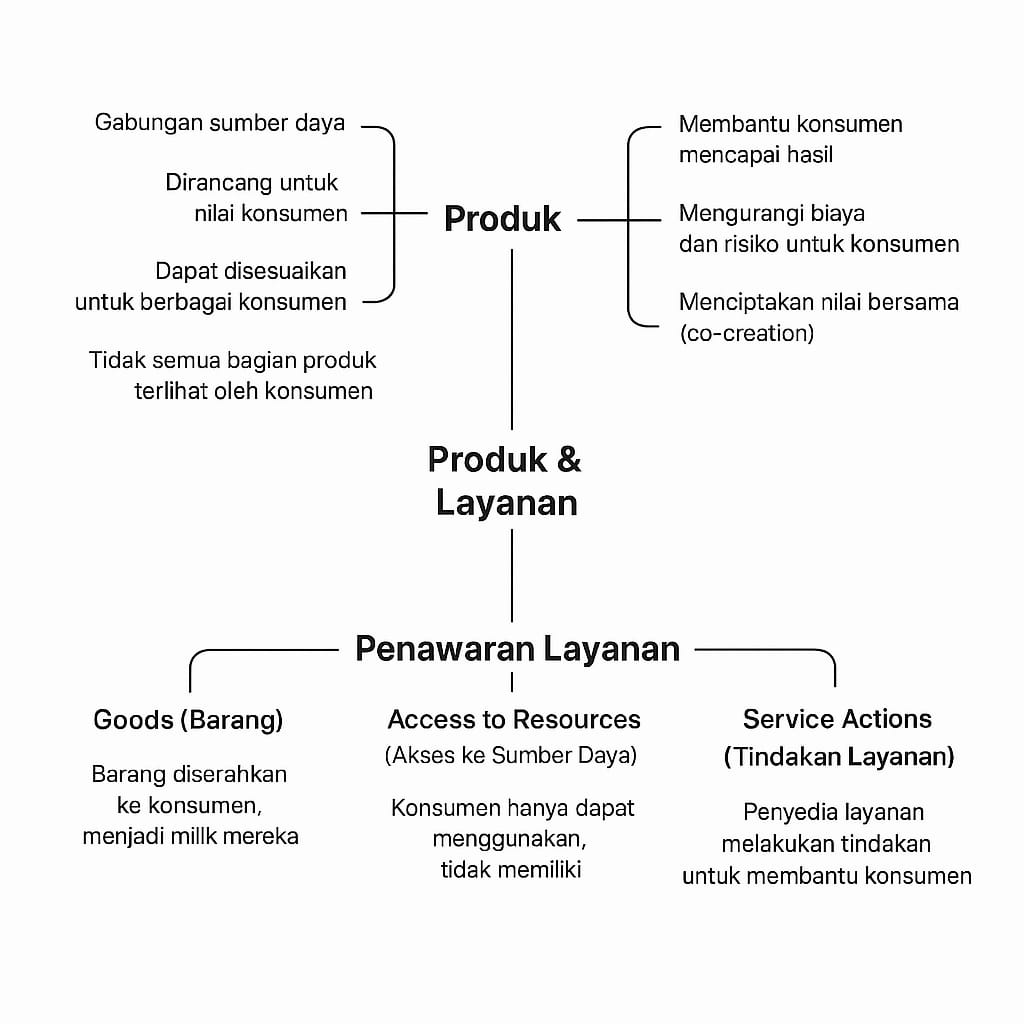
\includegraphics[width=0.5\linewidth]{Produk.jpg} % Ukuran gambar diperkecil
\end{frame}

% =====================================
% 9 - SECTION 5: Hubungan Layanan (Service Relationships)
% =====================================
\section{Hubungan Layanan (Service Relationships)}
\begin{frame}{Hubungan Layanan (Service Relationships)}
    Hubungan layanan terbentuk antara dua atau lebih organisasi untuk menciptakan nilai secara bersama-sama (co-create value). Dalam hubungan ini, organisasi dapat berperan sebagai penyedia layanan (service provider) maupun sebagai konsumen layanan (service consumer), bahkan bisa melakukan kedua peran sekaligus.
\end{frame}

\begin{frame}{Hubungan Layanan (Service Relationships)}
    \begin{block}{Model hubungan layanan}
    {Model ini terdiri dari tiga komponen utama}
        \begin{itemize}
            \item \textbf{Penyediaan layanan (Service Provision)}\\
            Kegiatan penyedia dalam mengelola sumber daya, memberikan akses, menjalankan layanan sesuai kesepakatan, dan perbaikan berkelanjutan.
            \item \textbf{Konsumsi layanan (Service Consumption)}\\
            Kegiatan konsumen dalam menggunakan layanan, mengelola sumber daya sendiri, serta meminta bantuan atau aksi dari penyedia layanan.
            \item \textbf{Manajemen hubungan layanan (Service Relationship Management)}\\
            Kegiatan kolaboratif antara penyedia dan konsumen untuk memastikan penciptaan nilai secara terus-menerus berdasarkan penawaran layanan yang disepakati.
        \end{itemize}
    \end{block}
\end{frame}

% =====================================
% 10 - SECTION 6: Nilai: Hasil, Biaya, dan Risiko
% =====================================
\section{Nilai: Hasil, Biaya, dan Risiko}
\begin{frame}{Nilai: Hasil, Biaya, dan Risiko}
    Bagian ini menjelaskan bahwa untuk mencapai hasil yang diinginkan, dibutuhkan sumber daya dan seringkali melibatkan risiko. Penyedia layanan membantu konsumen untuk mencapai hasil tersebut dengan mengambil sebagian biaya dan risiko, tetapi juga bisa memperkenalkan risiko dan biaya baru. Hubungan layanan hanya dianggap bernilai jika efek positifnya lebih besar dari efek negatifnya.
\end{frame}

\begin{frame}{Nilai: Hasil, Biaya, dan Risiko}
    \begin{block}{Hasil (Outcomes)}
        Merupakan hasil yang diharapkan oleh konsumen sebagai akibat dari layanan. Misalnya, mobil yang bersih dan terawat adalah output, sedangkan pengalaman perjalanan yang nyaman adalah outcome. Penyedia dan konsumen bisa bekerja sama dalam mendefinisikan outcome yang diinginkan.
    \end{block}
    \begin{block}{Biaya (Cost)}
        Adalah jumlah uang yang dikeluarkan untuk suatu aktivitas atau sumber daya tertentu.\\
        Terdapat dua tipe biaya dari sudut pandang konsumen:
        \begin{itemize}
            \item Biaya yang dihilangkan: biaya yang tidak lagi perlu ditanggung konsumen karena ditangani penyedia (contoh: tidak perlu membeli server sendiri).
            \item Biaya yang ditambahkan: biaya yang harus ditanggung konsumen untuk menggunakan layanan (contoh: biaya langganan, pelatihan staf).
        \end{itemize}
    \end{block}
\end{frame}

\begin{frame}{Nilai: Hasil, Biaya, dan Risiko}
    \begin{block}{Risiko (Risk)}
    Adalah kemungkinan kejadian yang dapat menyebabkan kerugian atau menyulitkan pencapaian tujuan.\\
    Risiko mencakup:
        \begin{itemize}
            \item Risiko yang dihilangkan oleh layanan (contoh: kehilangan data karena backup dilakukan penyedia).
            \item Risiko yang ditambahkan oleh layanan (contoh: ketergantungan pada satu vendor atau gangguan layanan dari pihak ketiga).
        \end{itemize}
        Konsumen juga berperan dalam mengurangi risiko dengan:
        \begin{itemize}
            \item Menyampaikan kebutuhan dan hasil yang diinginkan secara jelas.
            \item Memberi akses dan dukungan kepada penyedia layanan.
        \end{itemize}
    \end{block}
\end{frame}

\begin{frame}{Nilai: Hasil, Biaya, dan Risiko}
    \begin{block}{Utility dan Warrant}
    Konsep ini digunakan untuk menilai apakah layanan akan menciptakan nilai sesuai harapan.
        \begin{itemize}
            \item Utility adalah fungsionalitas yang ditawarkan oleh produk atau layanan untuk memenuhi kebutuhan. Dengan kata lain apakah layanan itu fit for purpose.
            \item Warranty adalah jaminan bahwa produk atau layanan akan memenuhi persyaratan yang disepakati. Dengan kata lain apakah layanan itu fit for use, mencakup aspek seperti ketersediaan, kapasitas, keamanan, dan kontinuitas.
        \end{itemize}
    \end{block}
\end{frame}

\begin{frame}{Nilai: Hasil, Biaya, dan Risiko}
    Semua elemen ini saling terkait dan harus dipertimbangkan bersama ketika menilai kelayakan dan nilai dari suatu layanan. Dengan memahami dan menyeimbangkan empat elemen di atas (outcome, cost, risk, utility, dan warranty), organisasi dapat menciptakan layanan yang benar-benar bernilai bagi konsumen maupun penyedia layanan itu sendiri. Contoh praktik seperti outsourcing cleaning service di Axle Car Hire menggambarkan bagaimana organisasi dapat menyeimbangkan outcome yang diharapkan, biaya yang ditanggung, dan risiko yang harus dikelola.
\end{frame}

% =====================================
% 11 - SECTION 7: PENUTUP
% =====================================
\section{Penutup}
\begin{frame}{Penutup}
    \begin{block}{Ringkasan (Summary)}
        \begin{itemize}
            \item Pentingnya memahami konsep nilai, produk, layanan, dan hubungan layanan dalam manajemen layanan.
            \item Menekankan bahwa manajemen layanan bukan sekadar memberikan layanan, tapi juga memastikan layanan tersebut memberikan manfaat nyata bagi konsumen.
            \item Organisasi harus fokus pada manfaat (benefits), biaya (costs), dan risiko (risks) untuk memastikan layanan yang diberikan benar-benar memenuhi kebutuhan pelanggan.
            \item Konsep ini akan dikembangkan lebih dalam di bab-bab selanjutnya.
        \end{itemize}
    \end{block}
\end{frame}

\begin{frame}{Penutup}
    \begin{block}{Simpulan (conclusion)}
        konsep penting dalam manajemen layanan, yaitu bagaimana nilai (value) diciptakan bersama (co-creation) antara penyedia dan konsumen layanan. Nilai bersifat subjektif dan dipengaruhi persepsi masing-masing pemangku kepentingan, termasuk organisasi, konsumen, dan pihak lain seperti pegawai dan mitra. Produk sebagai kombinasi sumber daya organisasi diubah menjadi penawaran layanan (service offerings) yang mencakup barang, akses ke sumber daya, dan tindakan layanan. Hubungan layanan dibangun melalui aktivitas penyediaan, konsumsi, dan manajemen hubungan layanan untuk mencapai nilai bersama. Layanan dinilai dari kemampuannya menghasilkan outcome yang diinginkan dengan pengelolaan biaya dan risiko yang baik, serta melalui konsep utility (kegunaan layanan) dan warranty (jaminan layanan).


    \end{block}
\end{frame}

\begin{frame}[standout]
  Ke warung beli es kelapa \\
  Diminum sambil duduk santai \\
  Kalau bisa jangan banyak tanya \\
  Biar kita cepat selesai
\end{frame}

% =====================================
% 12 - AKHIR DOKUMEN
% =====================================
\end{document}